%% [ADS 4-2005] Template file for 40in x 30in landscape poster
%%
%%
%%
%%
%% [ADS 4-2005] what follows here is obsolete I believe.
%%-------------------------------------------------------------------------
%% Written by Graeme, 2001-03 based on Norman's original microlensing
%% poster.
%%
%% $Id: poster-template-landscape.tex,v 1.1 2001/07/02 17:23:32 norman Exp $
%%
%% Default mode is landscape, which is what we want, however dvips and
%% a0poster do not quite do the right thing, so we end up with text in
%% landscape style (wide and short) down a portrait page (narrow and
%% long). Printing this onto the a0 printer chops the right hand edge.
%% However, 'psnup' can save the day, reorienting the text so that the
%% poster prints lengthways down an a0 portrait bounding box.
%%
%% 'psnup -w85cm -h119cm -f poster_from_dvips.ps poster_in_landscape.ps'
%%
%%-------------------------------------------------------------------------
%% Modified by Ronald Kumon, 06-2002 to incorporate a framebox border,
%%   add acknowledgments line at bottom, and change locations of logos
%%
%% Modified by Anand D. Sarwate 04-2005 to specialize to the UC Berkeley 
%%   EECS Wireless Foundaions conference poster template and for different
%%   paper sizes


%% [ADS 4-2005] latex --> dvips --> ps2pdf works just fine for me.
%%
%% To preview using xdvi:
%% 
%% $ xdvi -paper 1188x840mm -s 24 -nopostscript poster.dvi
%%
%% To convert dvi to Postscript:
%%
%% $ dvips -Ppdf -G0 -o poster.ps poster.dvi
%%
%% The dvips options are:
%% Ppdf: use the PDF printer configuration file
%% G0  : shift lower characters to higher position 
%%       (splits ligatures when using Times-Roman font)
%%
%% To convert Postscript to PDF:
%%
%% $ pstill -c -giptCQ -w 3368 -h 2378 -o poster.pdf poster.ps
%% ($ pstill -c -iptCQ -w 3225 -h 2378 -o poster.pdf poster.ps)
%%
%% Note that the pstill options are
%% c:  compression (more c's give more compression; up to four)
%% g:  take size from Postscript file
%% p:  include all fonts as partial fonts
%% i:  include all non-standard fonts
%% t:  map graphics transfer functions from PostScript to PDF. 
%% C:  use RGB color map
%% w:  width in points (1/72 inch) for 1188 mm
%% h:  height in points (1/72 inch) for 839 mm
%% Q:  take embedded fonts from PSFonts directory, not Postscript file
%% Note also that the -w and -h options need to be included else
%% some of the Postscript figures may not be displayed (particularly
%% those converted using fig2dev), even if the -g option is specified.
%% Also, the newest version of pstill (1.55.91) does not deal well with 
%% slanted Times Roman font; use italics or the older version (1.55.3). 
%%-------------------------------------------------------------------------


\documentclass{article}
%% [ADS 4/2005]  The template here does NOT make use of the 'slides'
%% option of Kumon in the interest of creating a more readable document
%% -- suggestions for how to make a backup style on separate sheet is
%% given in the text.
%%

%% If you want to number equations, set the equation number counter to zero.
%\setcounter{secnumdepth}{0}









%%%%%%%%%%%%%%%%%%%%%%%%%
%%% PACKAGE INCLUSION %%%
%%%%%%%%%%%%%%%%%%%%%%%%%

%% AMS packages for special symbols, etc
\usepackage{amsmath,amssymb}

%% This package gives you coloured text and various other simple
%% graphics hacks.  For details, see documentation in 
%% in /usr/local/teTeX/texmf/doc/generic/pstricks/*
\usepackage{pstricks}
\newrgbcolor{darkblue}{0.1 0.1 0.5}

%% The textpos package is necessary to position textblocks at arbitary 
%% places on the page.  Use showboxes option to show outlines of textboxes.
\usepackage[absolute]{textpos}
%\usepackage[absolute,showboxes]{textpos}

%% Package to include graphics.  
\usepackage{graphicx}
%% Define path for figures -- for safety, keep the last /
\graphicspath{./}

%% Wrap text around figures
%\usepackage{wrapfig}

%% Use Times font instead of Computer Modern -- this gives better
%% appearance when resizing to large sixes.
%% Note that without the ``G0'' in the dvips conversion, 
%% all character combinations that will normally result in 
%% ligatures will have to be hacked to display properly.  For example, 
%%     fi --> \mbox{f}\mbox{i}
%% Other characters may also fail.  In addition, the Mathtimes font 
%% set should really be used for mathematics, but unfortunately they 
%% are only proprietary.  (The Computer Modern fonts may still look OK.)
\usepackage{times}

%% These colors are tried and tested for titles and headers. Don't
%% over use color!
%\usepackage[usenames]{color} % commented by Karol Kozioł
\usepackage{xcolor}
\definecolor{DarkBlue}{rgb}{0.1,0.1,0.5}
\definecolor{Black}{rgb}{0.0,0.0,0.0}
\definecolor{Red}{rgb}{0.9,0.0,0.1}
\definecolor{DarkBlue2}{rgb}{0.00,0.08,0.6}
\definecolor{DarkRed2}{rgb}{0.6,0.00,0.08}
\definecolor{DarkGreen2}{rgb}{0.00,0.6,0.08}

%% Load shadow box package
%\usepackage{shadow}

%% This loads font sizes in style file a0size
\usepackage{a0size}

\usepackage[utf8]{inputenc}
\usepackage[english]{babel}


%%%%%%%%%%%%%%%%%%%%%%%%%%%%%%%% 
%%% NEW COMMAND DEFINTITIONS %%%
%%%%%%%%%%%%%%%%%%%%%%%%%%%%%%%%

%% See documentation for a0poster class for the size options here
%%    \normalsize will produce smaller type that might look too small
%%    \large will produce larger type
%% Feel free to modify if you want a different look
\let\Textsize\normalsize
%\let\Textsize\large
\def\RHead#1{\noindent\hbox to \hsize{\hfil{\LARGE\color{DarkBlue} #1}}\bigskip}
\def\LHead#1{\noindent{\LARGE\color{DarkBlue} #1}\bigskip}
\def\CHead#1{\begin{center}\noindent{\LARGE\color{DarkBlue} #1}\end{center}}
\def\Subhead#1{\noindent{\large\color{DarkBlue} #1}\bigskip}
\def\Title#1{\noindent{\textbf{\veryHuge\color{Red} #1}}}




%%%%%%%%%%%%%%%%%%%%%%%%%%%%%
%%% GLOBAL LAYOUT OPTIONS %%%
%%%   NUMBER OF COLUMNS   %%%
%%%%%%%%%%%%%%%%%%%%%%%%%%%%%

%% Set paper size
%% Depending on the conference, the posterboard size may be different.
%% This template was based on an ISO standard A0, which is in use everywhere
%% except for the United States.  A0 paper is  46.81 in x 33.11 in.
%% Depending on the posterboard size and the printer, you may need to 
%% change the widths and margins here.  Text width and height are set
%% in terms of paper width and height -- you can change margins here.
\setlength{\paperwidth}{40in}
\setlength{\paperheight}{30in}
\setlength{\textwidth}{36in}    %% paperwidth - (3in)
\setlength{\textheight}{26in}   %% paperheight - (3in)
\special{papersize=\the\paperwidth,\the\paperheight}
\typeout{Paper width and height are \the\paperwidth and \the\paperheight}
\typeout{Text width and height are \the\textwidth and \the\textheight}
%% Margins
\setlength{\headheight}{0cm}
\setlength{\headsep}{0cm}
\setlength{\topmargin}{1in}
\setlength{\topskip}{0cm}
\setlength{\oddsidemargin}{1in}
\setlength{\evensidemargin}{0in}
%% Font sizes
\renewcommand{\tiny}{\fontsize{12}{14}\selectfont}
\renewcommand{\scriptsize}{\fontsize{14.4}{18}\selectfont}   
\renewcommand{\footnotesize}{\fontsize{17.28}{22}\selectfont}
\renewcommand{\small}{\fontsize{20.74}{25}\selectfont}
\renewcommand{\normalsize}{\fontsize{24.88}{30}\selectfont}
\renewcommand{\large}{\fontsize{29.86}{37}\selectfont}
\renewcommand{\Large}{\fontsize{35.83}{45}\selectfont}
\renewcommand{\LARGE}{\fontsize{43}{54}\selectfont}
\renewcommand{\huge}{\fontsize{51.6}{64}\selectfont}
\renewcommand{\Huge}{\fontsize{61.92}{77}\selectfont}
\newcommand{\veryHuge}{\fontsize{74.3}{93}\selectfont}
\newcommand{\VeryHuge}{\fontsize{89.16}{112}\selectfont}
\newcommand{\VERYHuge}{\fontsize{107}{134}\selectfont}
%% skip lengths
\setlength{\smallskipamount}{6pt plus 2pt minus 2pt}
\setlength{\medskipamount}{12pt plus 4pt minus 4pt}
\setlength{\bigskipamount}{24pt plus 8pt minus 8pt}
\setlength{\abovecaptionskip}{25pt}
\setlength{\belowcaptionskip}{0pt}
\setlength{\abovedisplayskip}{25pt plus 6pt minus 15 pt}
\setlength{\abovedisplayshortskip}{0pt plus 6pt}
\setlength{\belowdisplayshortskip}{13pt plus 7pt minus 6pt}
\setlength{\belowdisplayskip}{\abovedisplayskip}

%% Set up the grid
%%
%% Note that [40mm,40mm] is the margin round the edge of the page
%% it is _not_ the grid size. That is always defined as 
%% PAGE_WIDTH/HGRID and PAGE_HEIGHT/VGRID. In this case we use
%% 46 x 26. This gives us 4 columns of width 10 boxes, with a gap of
%% width 2 in between them.  There are 26 vertical boxes.
%%
%% (Note however that texblocks can be positioned fractionally as well,
%% so really any convenient grid size can be used.)
%%
\TPGrid[40mm,40mm]{46}{26}      % 4 cols of width 10, plus 3 gaps width 2

%% Text layout parameters
\parindent=0pt
\parskip=0.5\baselineskip





%%%%%%%%%%%%%%%%%%%%%
%%% THEOREMS, ETC %%%
%%%%%%%%%%%%%%%%%%%%%
\newtheorem{thm}{Theorem}






%%%%%%%%%%%%%%%%%%%%%%%%%%%%
%%% DOCUMENT BEGINS HERE %%%
%%%%%%%%%%%%%%%%%%%%%%%%%%%%

%% The basic format of the poster is to create text boxes with the
%% various things you want to display.  You can then play around 
%% with how to lay thing out.  In the old version of this template,
%% the content was always provided with alternatives suitable for
%% printing on sheets of paper (resizing fonts, images, etc).  I
%% think that's too confusing to read.  The old layout was:
%%     \ifposter
%%          some poster commands go here
%%     \else
%%          an alternative style here in case you are printing on
%%          regular sheets of paper
%%     \fi
%% One option is to make the entire poster and then wrap it in an \ifposter
%% and then make all the slides separately.  This seems to be easier
%% if your poster is not much like a bunch of 8.5x11 sheet tacked together
%% in the first place.
\begin{document}

%% Do not put page numbers at the bottom of the page for poster
\pagestyle{empty}



%% Declare proper hyphenation
\hyphenation{equi-bi-ax-i-al}
\hyphenation{in-fin-i-tes-i-mal}


%% Border and background options -- you can make up others if you
%% like.  These all use the pstricks package.
%% DRAW A BLUE BORDER AROUND THE POSTER USING PSTRICKS
\psset{linewidth=0.5cm}
% Sets up lengths for frame
\newlength{\frameleft}
\newlength{\frameright}
\newlength{\frametop}
\newlength{\framebottom}
\setlength{\frameleft}{-1in}
\setlength{\frameright}{\textwidth}
\addtolength{\frameright}{1in}
\setlength{\frametop}{1in}
\setlength{\framebottom}{-\textheight}
\addtolength{\framebottom}{-1in}
% Draws a blue frame
\psframe[linecolor=darkblue,cornersize=absolute,linearc=2]
(\frameleft,\framebottom)(\frameright,\frametop)% need to overlay EOSMLS
%\psline{->}(0cm,0cm)(\textwidth,-\textheight)
%   *** End code to draw border *** 

%% USE A COLORED BACKGROUND FOR THE ENTIRE POSTER
%% [ADS 4-2005] THIS OPTION IS NOT SUPPORTED YET
%\newrgbcolor{gradbegin}{0.3 0.5 0.7}
%\newrgbcolor{LightBlue}{0.7 0.7 1.0}
%\psframe[fillstyle=solid,fillcolor=LightBlue](\frameleft,\framebottom)(\frameright,\frametop)



%% Adjust spacing in long displayed mathematical formulas to tighten them up
\setlength{\abovedisplayskip}{0.75\abovedisplayskip}
\setlength{\belowdisplayskip}{0.75\belowdisplayskip}



%% Understanding textblocks is the key to being able to do a poster in
%% LaTeX. The first argument gives the block width in grid cells, the
%% second gives the positioning on the grid.
%%
%% NOTE:  You will have to do a lot of previewing to get everything
%% in the right place.
%%
\begin{textblock}{46}(00,00)
\begin{center}
\Title{Modeling ODE Systems - A Pine Beetle Dispersion Analysis}
\end{center}
\end{textblock}

\begin{textblock}{46}(00,01.5)
\begin{center}
\LHead{Lucas Wilson}\\
\LHead{\textit{Math 451: Numerical Analysis II - Modeling ODE Systems - A Pine Beetle Dispersion Analysis}}
\end{center}
\end{textblock}


%% UCB EECS logo on left, Wireless Foundations Logo on right
\begin{textblock}{8}(00.5,01)
\begin{center}
%\includegraphics[height=5cm]{eecs.eps}
%TODO
\end{center}
\end{textblock}

\begin{textblock}{8}(38,01)
\begin{center}
%\includegraphics[height=5cm]{wifound.eps} % modified by Karol Kozioł
%\includegraphics[height=2.5cm]{wifound.eps}
%TODO
\end{center}
\end{textblock}


\begin{textblock}{42}(02,03)
\begin{center}
\rule{1200pt}{7pt}
\end{center}
\end{textblock}



%% Begin 1st row
\begin{textblock}{10}(00,04)
\CHead{Introduction}            %% \CHead creates a centered title
\begin{itemize}
\item The goal of this project is to create a basic mathematical model of the dispersion of Mountain Pine Beetles using a system of ODEs.
\item The model is calculated numerically using a fourth order Runge-Kutta method. I analyze the cost of calculating the model and the accuracy. I also look at the error of using the same time step with a lower order Runge-Kutta method.
\item I vary carrying capacity, emigration/immigration rates, and the different starting conditions to analyze different effects they have.
\end{itemize}
\end{textblock}



\begin{textblock}{10}(00,10)
\CHead{Motivation}
Mountain Pine Beetles infesting our trees is an important problem today. We depend heavily on our already limited trees, and the beetles are destroying that resource. Although this model doesn't take it into account, trees do die when infected with enough beetles. Learning how they spread can help us know the most effective way to eradicate or servery mitigate them.
\end{textblock}


\begin{textblock}{10}(00,14)
\CHead{Mathematics}
I assume trees in a forest are evenly distributed in a grid (to reduce computational complexity). I assume there are four methods for beetles to spread and emerge: birth rate, death rate, immigration rate and emigration rate.
\begin{itemize}
\item Birth and death rate are modeled with a logistic model:\\
$P(x) = px(1-\frac{x}{C})$ where $C =$ carrying capacity, and $p$ is the population rate proportion.
\item Emigration is proportional to the population:\\
$E(x) = ex$ where $e =$ the emigration proportion.
\item Immigration is proportional to the sum of all other tree's emigration decayed with distance.\\
$M(x_i) = m\sum_{i \neq j}^{n}\frac{E(x_j)}{dist(i, j)}$ where $dist(i, j)$ is the euclidean distance between tree $i$ and $j$, and $m$ is the immigration proportion (since not all that reach the tree infect the tree).
\end{itemize}
The rate of change in population of Mountain Pine Beetles in a tree is proportional to each of these.\\
$\frac{dx}{dt} = P(x) + E(x) + M(x)$ where $x = (x_1, x_2, ..., x_n)^T$ and $x_i$ is the number of beetles in tree $i$.\\
Runge-Kutta is an explicit method of calculating $x$ after $\Delta t$ seconds derived from a taylor expansion:\\
$x^{(k)} = f(t^{(k-1)}, x^{(k-1)})$ or $x(t+\Delta t) = f(t, x(t))$\\
A fourth order Runge-Kutta uses the fourth order terms of a Taylor Series, so the err is of 5th order: $O(\Delta t^5)$.
\end{textblock}



\begin{textblock}{10}(12,04)
\CHead{Evaluation of Solution}
For $\Delta t, x^{(k)} = u + Ch^5$, and
for $\frac{\Delta t}{2}, x^{(k)} = v + 2C\frac{h}{2}^5$\\
Solving for $Ch^5$ shows that error is proportional to $x_{\Delta t}^{(k)}-x_{\frac{\Delta t}{2}}^{(k)}$. Thus, if $x_{\frac{\Delta t}{n}}^{(k)}$ converges, then the error converges.\\
Using $\Delta t_i = \frac{1}{100*2^i}$ and finding $||x_{\Delta t_i}^{(k)}-x_{\Delta t_{i-1}}^{(k)}||_{\inf}$ yields\\
$error = 0.124, 0.0618, 0.0308, 0.0153$.\\
Notice that the $Ch^5$ approximations are approaching zero (proportionally to $\Delta t$). Therefore, Runge-Kutta converges and is a valid method for numerically calculating my beetle model.
\end{textblock}




\begin{textblock}{10}(12,19)
\CHead{Lower Order Runge-Kutta Methods}

In order to analyze the effectiveness of lower order Runge-Kutta methods, we will use fourth order (RK-4) as a baseline and look at new error and the performance increase of second order (RK-2). My analysis shows that RK-2 can be used as a performance increase with small error.
\begin{itemize}
\item A time analysis shows that computational time cost of RK-4 and RK-2 are proportional to $\Delta t$ and RK-2 is about 6 times faster.
\item Performing the same error analysis as above shows that RK-2 also converges.
\item Using $\Delta t = 3.125e-4, x^{(k)}_{RK-4} - x^{(k)}_{RK-2} = 6.43e-6$. 
\end{itemize}
\end{textblock}




\begin{textblock}{10}(24,04)
\CHead{Vary Starting Conditions}
Changing the starting conditions has no effect on the long term distribution of the beetles. The beetles migrate towards the center with time. The reason for this is because the emigration and immigration rate reach an equilibrium. Trees in the center of the forest are closest to all trees, thus more beetles emigrating from other trees can reach it more easily while edge trees are less exposed to migrating beetles.
\end{textblock}



\begin{textblock}{22}(12,9)
\CHead{Base Model and with Varying Initial Conditions}
\begin{center}
%\includegraphics[width=18in]{samplefig.eps}
%TODO
\end{center}
\end{textblock}



\begin{textblock}{10}(24,19)
\CHead{Time Complexity vs $\Delta t$}
\begin{figure}[htp]
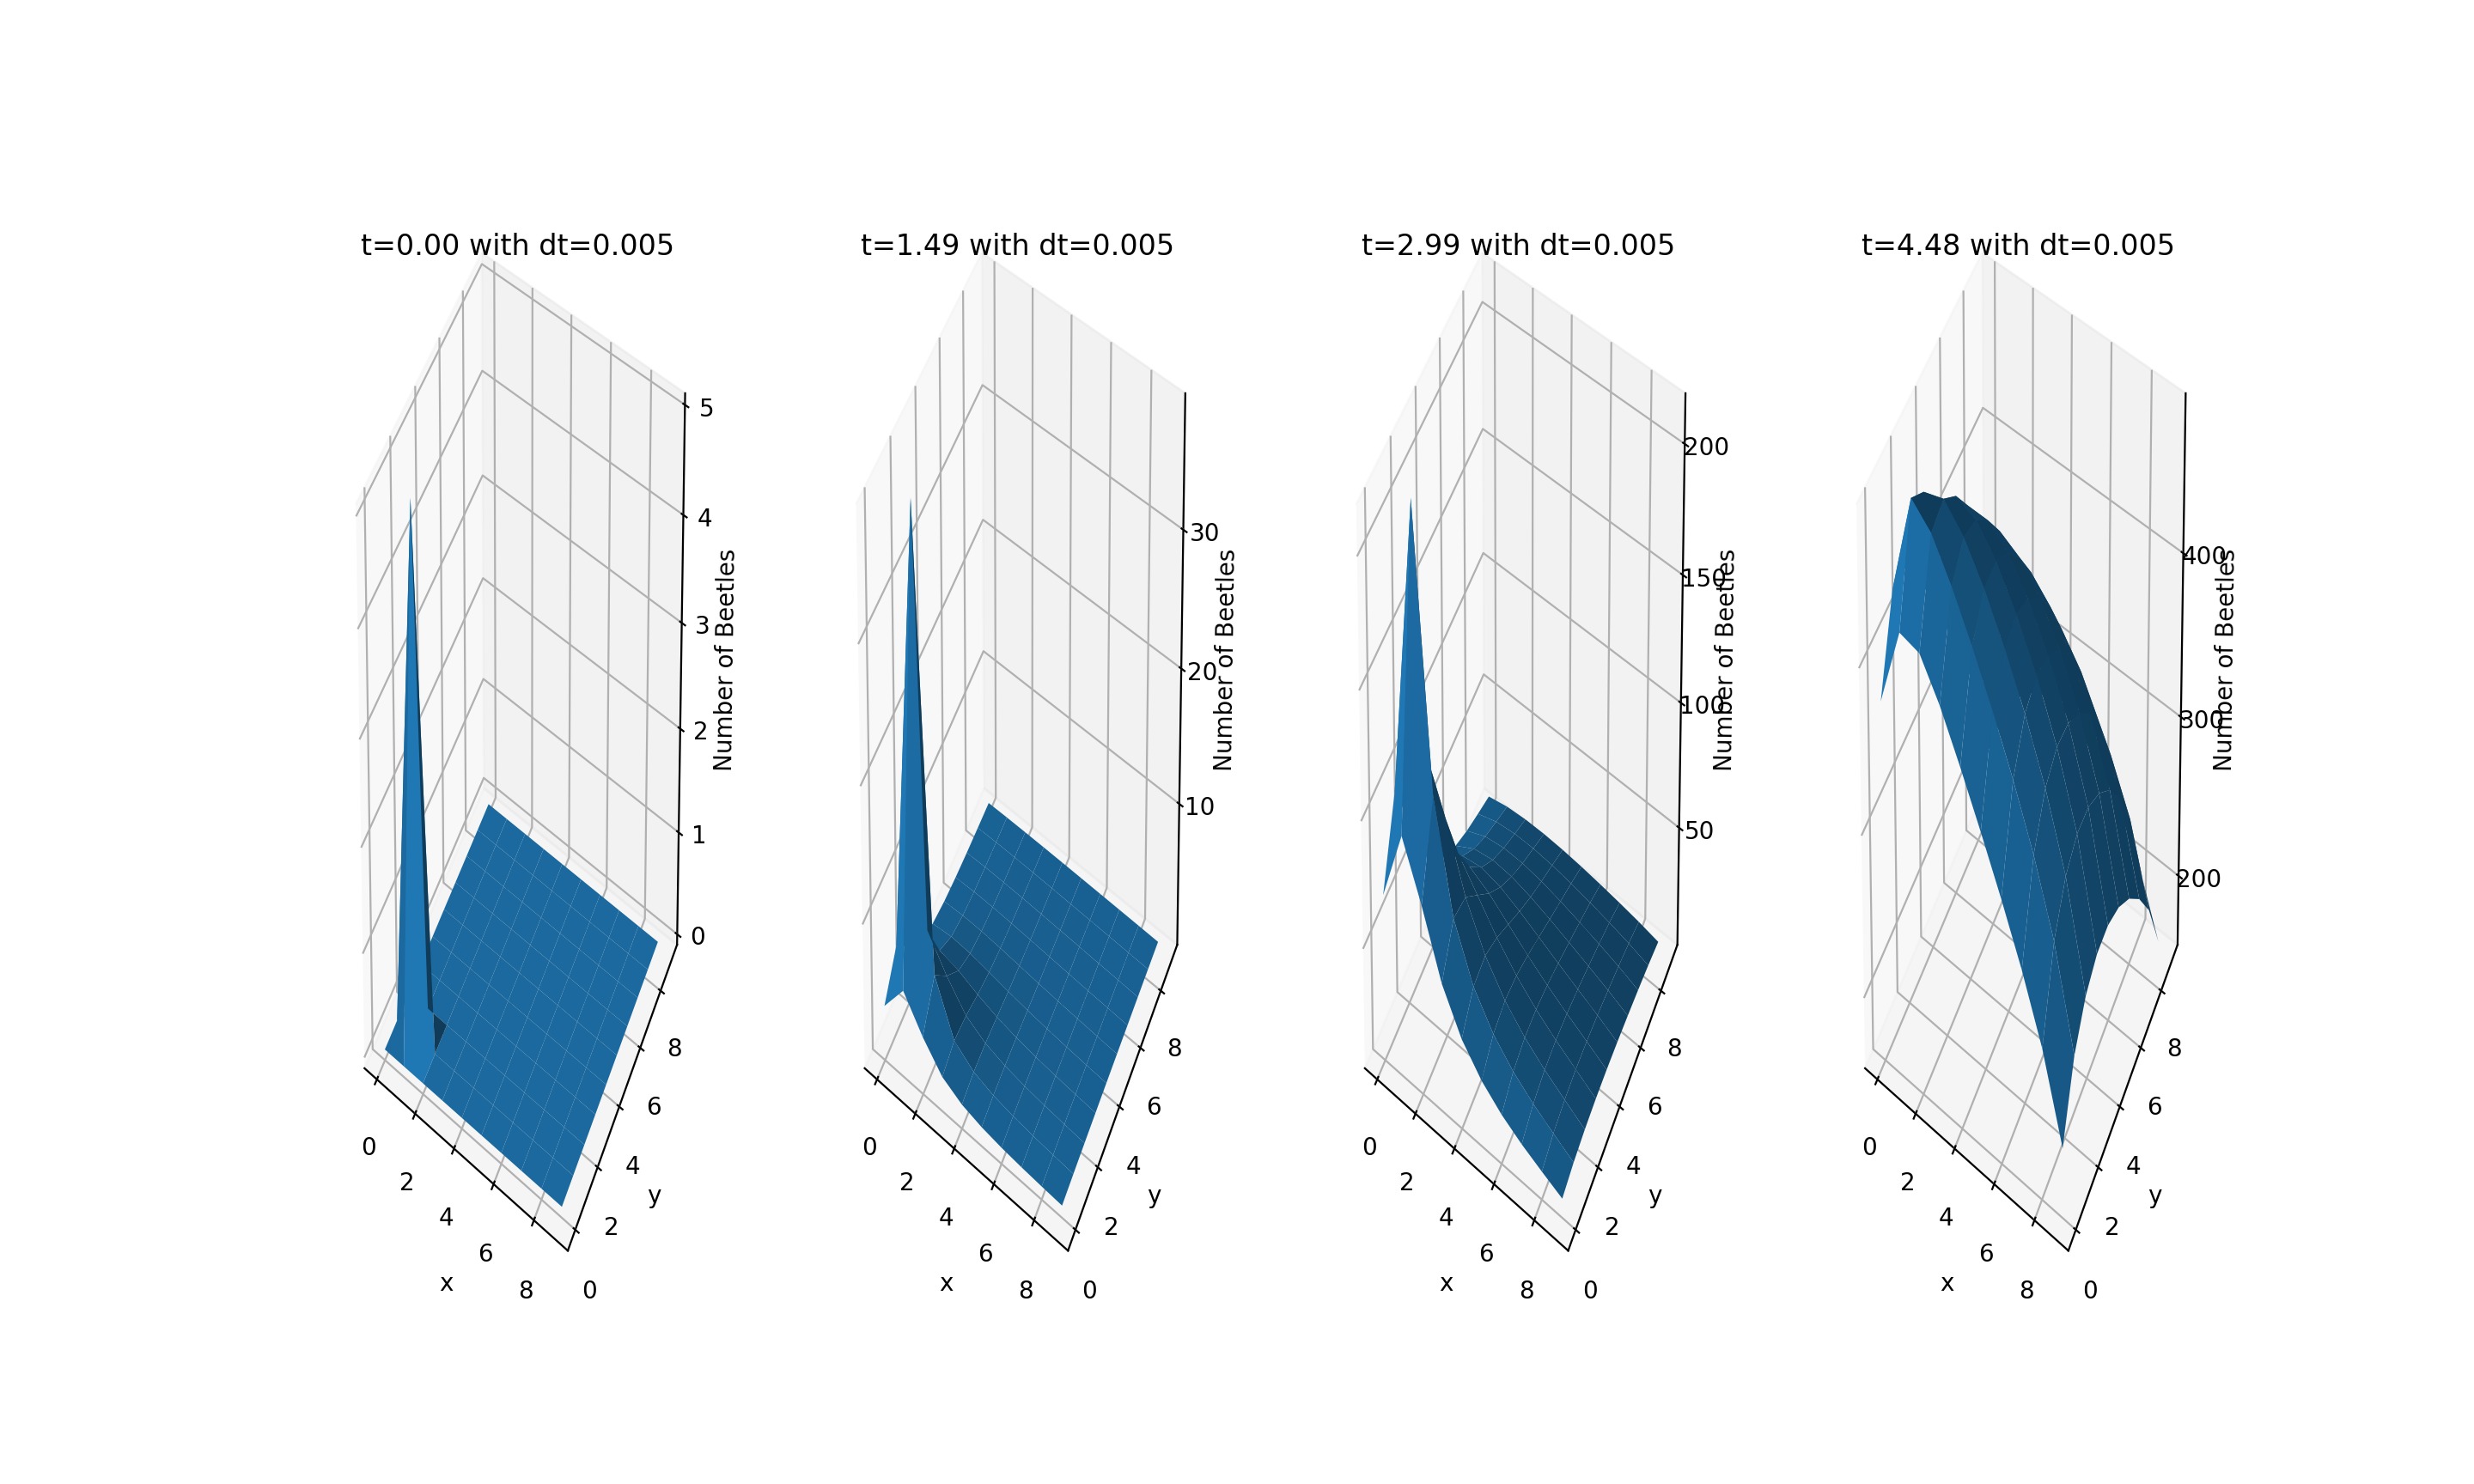
\includegraphics[width=\linewidth]{base}
\end{figure}
\end{textblock}


\begin{textblock}{10}(36,04)
\CHead{Mitigating Reproduction Rate}
Mitigating the reproduction rate causes the beetles to spread much more slowly and limits the ability for the beetles' population to grow within a specific tree. From the graph, we can see that the total number of beetles in even the starting tree is much lower than the base model. Since there are fewer beetles in total, there are fewer spreading to other trees.\\
This can be good or bad. It does mitigate the spread of beetles, and it also keeps the trees alive. Although the trees are alive, they are still spreading the beetles. Thus, beetles can spread to the entire forest. If at some point, they are able to reproduce to the point of killing a tree, the entire forest will die since every tree is infected.\\
Overall, mitigating reproduction ability reduces the total number of beetles within each tree.
\end{textblock}


\begin{textblock}{10}(36,15)
\CHead{Mitigating Immigration/Emigration Rate}
Mitigating the beetles' ability to migrate from tree to tree has the effect of keeping the infestation very localized. The beetles spread very slowly throughout the forest. This is very similar to the situation of mitigating reproduction rate with the exception of the beetle population within each tree. As the beetle population increases, the number migrating also increases finally allowing beetles to spread to other trees.\\
However, if we consider the fact that a large amount of beetles will kill the tree and thus the beetles, then beetles will die before being capable of spreading to other trees. This causes the beetle infestation to be very localized.\\
Overall, the mitigation of immigration/emigration rates is very effective in fighting the beetles assuming the tree dies before beetles can successfully spread.
\end{textblock}


%\begin{textblock}{10}(36,21)
%\bibliographystyle{plain}
%\bibliography{posterTemplate}
%\end{textblock}



%\begin{textblock}{46}(00,25.5)
%\begin{center}
%{\footnotesize Contact information:
%Anand D.~Sarwate, 264 Cory Hall, Department of EECS, University of California, Berkeley, %Berkeley, CA 94720\ \ --
%Phone: 510--643--9263\ \ -- 
%Email: \textit{asarwate@eecs.berkeley.edu}; 
%Web: \textit{http://www.eecs.berkeley.edu/}
%}
%\vspace{-0.75\baselineskip}
%
%{\footnotesize Acknowledgments: This work was performed while the
%author held a National Defence Science and Engineering Graduate
%Fellowship.  This template was modified only slightly from that of Ron
%Kumon in order to make it more specifically a tutorial for the
%Berkeley Wireless Foundations Center.}
%\end{center}
%\end{textblock}

\end{document}

